\chapter{Benchmarks}

In this chapter, we present two benchmarks, which explore the used technology limitations.
We introduce the background of the benchmarks, execute them and then evaluate the results.

\section{Rendering}

This benchmark observes the limitation of a page refreshing using two ways for rendering a page content.
We modify the \texttt{Asteroids} game, mentioned earlier, to explore FPS during rendering.
The modified application generates asteroids, represented by \texttt{<div>} element with CSS styles, and lets them fall until they reach the bottom, as we can see in Figure \ref{img33:benchmark}.
Then, they are removed.
We log the current FPS, count of elements generated by the application, and time from starting the measurement every second.
Then, we evaluate the results.
\par
\begin{figure}[b!]\centering
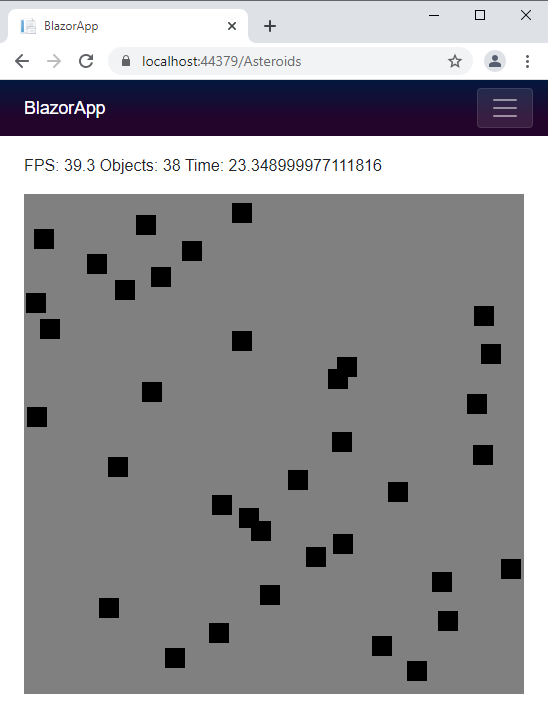
\includegraphics[scale=0.7]{./img/BenchmarkRendering}
\caption{The example.}
\label{img33:benchmark}
\end{figure} 
\par
This benchmark is created as a separated .NET solution, \texttt{Rendering}.
The solution consists of three projects: \texttt{BlazorApp.Client}, \texttt{BlazorApp.Server}, \texttt{PHPScripts}.
The setting of BlazorApp is similar to the previous demo.
\texttt{PHPScripts} contains the modified game together with additional scripts providing the interactive setting for the benchmark in a browser.
When we start the server and navigate the website, we can set various properties of measurement like an FPS, a frequency of asteroids, or dimensions of background.
We will explain only the \textit{Rendering} property because the rest of the properties are self-explaining.
We have two options for the property.
We call the first one \texttt{Simple} rendering because it uses \texttt{AddMarkup} method for updating the page content.
This method accumulates the generated HTML entities into a single string and adds it into \texttt{PhpTreeBuilder}.
We call the second one \texttt{Complex} rendering because it utilizes specialized builder interface for adding HTML entities, which includes \texttt{AddAttribute} for example.
\par
We suppose that the first method is less effective than the second because the diff algorithm makes lesser update optimizations in the first case.
It is caused by not providing the sequence numbers for each of the HTML entities, but it is regarded as the one part.
This part is regenerated every time instead of update only the changed parts.
\par
The following benchmarks uses Google Chrome (version: 90.0.4430.93) browser.
We used notebook with Intel(R) Core(TM) i7-8550U CPU, 8GB RAM, and NVIDIA GeForce MX150.
\par
We can see results from the first measurement in Figure \ref{img31:benchmark1}.
We set the timer to refresh the window sixty times per second, which results in 60 FPS.
Then, we generate five asteroids per second.
The dimensions of the background are 800 x 800.
We measure the FPS and number of objects for 60 seconds.
We can see two graphs displaying the current time and number of objects.
The lines represent measured values for each type of rendering.
\par
The second measurement aims at the deeper structure of updating elements. 
It should magnify the difference between the first and the second way.
We create an asteroids as \texttt{<div>} element containing inner three \texttt{<div>} elements, which have one \texttt{<div>} element.
These elements have no special styles, just simulates a complex structure.
So the one asteroid consists of nine HTML elements.
The setting is the same as the previous one.
\par
\begin{figure}\centering
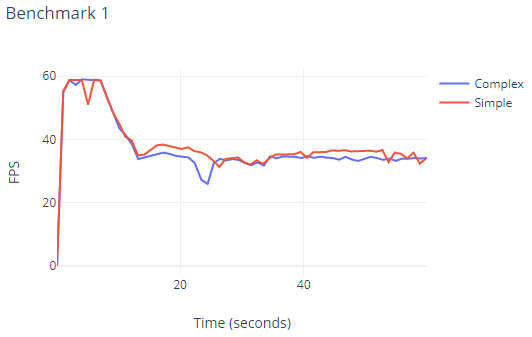
\includegraphics{./img/graph_1}
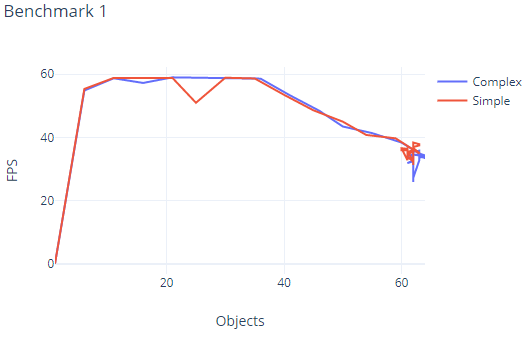
\includegraphics{./img/graph_2}
\caption{FPS: 60, Asteroids Per Second: 5, Background dimensions: 800x800, Duration: 60, Asteroid size: 20, Asteroid speed (Pixels Per Second): 60 , one element per Asteroid}
\label{img31:benchmark1}
\end{figure} 
\par
\begin{figure}\centering
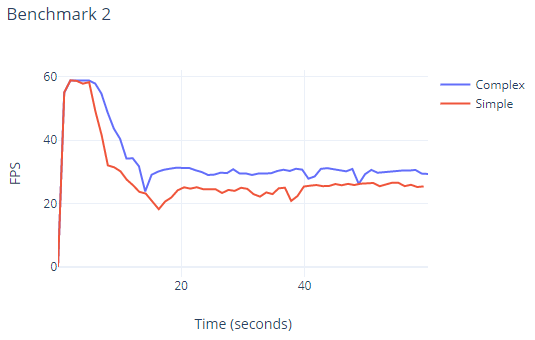
\includegraphics{./img/graph_4}
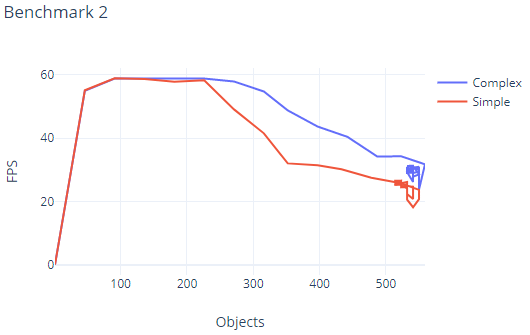
\includegraphics{./img/graph_3}
\caption{FPS: 60, Asteroids Per Second: 5, Background dimensions: 800x800, Duration: 60, Asteroid size: 20, Asteroid speed (Pixels Per Second): 60 , nine elements per Asteroid}
\label{img32:benchmark2}
\end{figure} 
\par
We can see that when the updating objects have not inner elements, the rendering ways are similar.
When the updated objects have inner elements, the FPS is lower in the first way of rendering, as we can see in Figure \ref{img32:benchmark2}.
This is caused by optimized updates made by the diff algorithm, which generates only DOM updates for the element style and leaves the inner tree unchanged.
As we can see, the FPS is aboat 29 in the second way, which is fine because the untrained eye is able to distinguish up to 23 images per second.
The first way has about 20 FPS per second most of the time, which looks glitchy in the browser.
This benchmark gives reasons for using the builder properly and the need to use \texttt{PhpComponent} for render demanding applications.
\par
Another problem caused by the first way of rendering is handling click events when the window is being quickly refreshed.
Because the click events consist of two inner events (mouse up, mouse down), the event is not fired due to removing the element before the second event appears.

\section{GD library}

This benchmark tests the effectivity of PHP library, \textit{gdlibrary}, in the Blazor environment.
We prepare a simple script, which creates a blank image with 1920x1080 resolution.
We use \texttt{imagecreatetruecolor} function defined in the library.
Then we measure elapsed time during the function execution by printing the current time before and after the function call.
We compare the results with executing the script in a desktop environment, where we use Peachpie and native PHP interpreter.
\par
The benchmark is created as a .NET solution consisting of four projects: \texttt{BlazorApp.Client}, \texttt{BlazorApp.Server}, \texttt{Desktop}, \texttt{PHPScripts}.
The \texttt{PHPScripts} project contains \textit{index.php}, which does the benchmark.
The \texttt{Desktop} project runs the script in a console application.
\texttt{BlazorApp} projects run the script in a browser.
The benchmark uses Google Chrome (version: 90.0.4430.93) browser and Apache server.
We used notebook with Intel(R) Core(TM) i7-8550U CPU, 8GB RAM, and NVIDIA GeForce MX150.
\par
We can see the result of measurement in table \ref{tab01:time}.
The difference between the execution with a native interpreter and the console application is caused by using the different graphic libraries.
Peachpie uses the \texttt{ImageSharp} library, which is a graphic library written in C\#.
The native interpreter uses a different library written in C.
The execution interpreter is the fastest.
However, we consider the execution times of the results almost the same.
The suprising thing is the execution time in the browser environment, which is extensively worse.
We suppose that it is caused by the \texttt{ImageSharp} library, which has not to be optimized in the browser environment.
\par
\begin{table}[b!]
\centering
\begin{tabular}{l@{\hspace{1.5cm}}D{.}{,}{3.2}D{.}{,}{1.2}D{.}{,}{2.3}}
\toprule
\mc{\textbf{Enviroment}} & \mc{\textbf{Execution time (seconds)}}\\
\midrule
Blazor - Peachpie  & \mc{23,56} \\
Desktop - Peachpie & \mc{0,22} \\
Desktop - Native   & \mc{0,002} \\
\end{tabular}
\caption{Elapsed time of the function execution.}
\label{tab01:time}
\end{table}
\par

